\documentclass[12pt]{article}

% \usepackage[default]{sourcecodepro}
% \usepackage[T1]{fontenc}

\usepackage{amsfonts, lipsum}
\usepackage{amsmath,amssymb, amscd,amsbsy, bbm, amsthm, enumerate}
\usepackage{mdframed, titlesec, setspace,verbatim, multicol}
\usepackage[top=1in, bottom=1in, left=.45in, right=.45in]{geometry}
\usepackage[unicode]{hyperref}
\usepackage{tikz, pgfplots, xcolor, fancyhdr}
\usepackage{graphicx, caption, subcaption}
\usepackage{stmaryrd}

\setlength{\parindent}{0pt}
\setlength{\textheight}{9in}

%%% Header and Footer Info
\pagestyle{fancy}
% \fancyhead[L]{{\large CSE431 Assignment 4}}
% \fancyhead[C]{}
% \fancyhead[R]{Name: Bradley Bauer}
\fancyhead[L]{\large CSE 431 Assignment 4 }
\fancyhead[C]{}
\fancyhead[R]{\large Question 1}

\theoremstyle{definition}

%%% These are some shortcuts that are handy
\def\real{{\mathbb R}}
\def\Natural{\mathbb{N}}
\def\dx{\textnormal{dx}}
\def\dy{\textnormal{dy}}
\def\dz{\textnormal{dz}}
\def\dt{\textnormal{dt}}
\def\ds{\textnormal{ds}}
\def\dw{\textnormal{dw}}
\def\Re{\textnormal{Re}}
\def\Im{\textnormal{Im}}
\def\exp{\textnormal{exp}}
\def\interior{\textnormal{interior}}
\def\al{\alpha}
\def\del{\delta}
\def\Del{\Delta}
\def\gam{\gamma}
\def\Gam{\Gamma}
\def\Om{\Omega}
\def\ep{\varepsilon}
\def\lam{\lambda}
\def\rational{{\mathbb Q}}
\def\integer{{\mathbb Z}}
\def\Q{{\mathbb Q}}
\def\Z{{\mathbb Z}}
\def\N{{\mathbb N}}
\def\R{{\mathbb R}}
\def\grad{\nabla}
\def\C{\mathcal C}
\def\P{\mathcal P}
\def\T{\mathcal T}
\def\I{\mathcal I}
\newcommand{\abs}[1]{\left| #1 \right|}
\newcommand{\inner}[1]{\langle #1 \rangle}
\newcommand{\norm}[1]{\left\lVert#1\right\rVert}
\newcommand{\spanvect}{\textnormal{span}}
\newcommand{\union}{\cup}
\newcommand{\Union}{\bigcup}
\def\intersect{\cap}
\def\Intersect{\bigcap}

\newtheorem{innercustomthm}{}
\newenvironment{question}[1]
  {\renewcommand\theinnercustomthm{#1}\innercustomthm}
  {\endinnercustomthm}

\begin{document}

\begin{question}{Hypothesis}
    Insertion sort is faster than quicksort for input arrays of size 50 or smaller.
\end{question}

\begin{question}{Methods}
    The experiment is ran on Ubuntu 19.04. GCC version is 8.3 and python version is 3.7.3.
    Also, matplotlib is a dependency of plot.py\\\\
    To run the experiment, first compile
    $$\text{g++ -fconcepts -std=c++2a -O3 code.cpp}$$
    Then execute $$\text{./a.out}$$
    To plot the results use
    $$\text{python3 plot.py}$$
    The code runs quicksort and insertion sort on arrays, of length n=1,\dots,400, containing uniform random integers from the range [0,2147483647].
    For each input size n, the algorithms are tested on 10000 random input arrays of length n and the results are averaged.
    This produces n pairs of numbers.
    The ith pair of numbers, call it (a,b), represents a:$\;$the average time taken for quicksort on uniform random inputs of size i, and b:$\;$the average time taken for insertion sort on uniform random inputs of size i.
\end{question}

\newpage
\begin{question}{Results}
$\\$
\vspace{-1cm}
\begin{figure}[h]
  \centering
  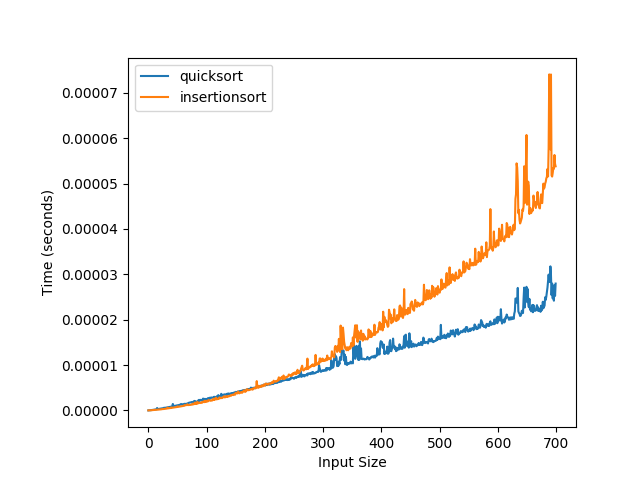
\includegraphics[width=\textwidth]{Figure_1.png}
  \caption{}
  \label{fig:boat1}
\end{figure}

\begin{figure}[h]
  \centering
  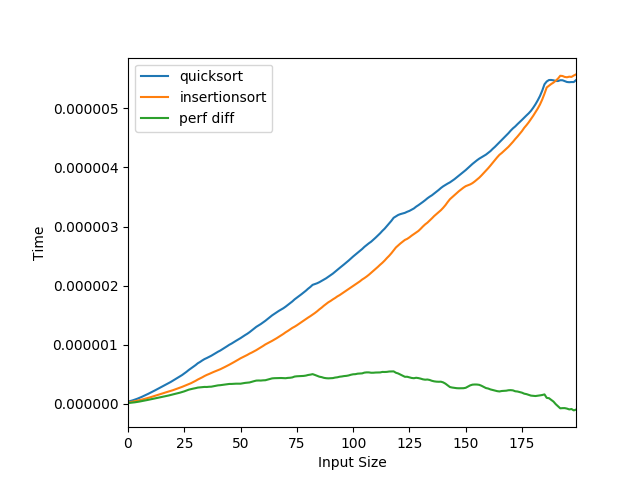
\includegraphics[width=\textwidth]{Figure_2.png}
  \caption{}
  \label{fig:boat2}
\end{figure}

Figure 1 shows a plot of the n pairs of numbers described above.
\newpage
Figure 2 is a zoomed in plot of the data in Figure 1, but with an additional curve showing the difference in performance for quicksort and insertionsort.

\end{question}

\begin{question}{Discussion}
    Figure 2 shows that quicksort takes the lead around input size 180.
    One thing to note is that the maximum performance difference between quicksort and inesrtionsort is somewhere between 75 and 115.
\end{question}

\begin{question}{Conclusion}
  Quicksort is faster than insertion sort for n>180.
\end{question}

\end{document}
